\documentclass[tikz,border=3pt]{standalone}

\usepackage{wit-graphics-2012}
\usepackage{wit-code-2012,calc}
\usetikzlibrary{calc}

\usepackage{relsize}

\tikzstyle{cell}=[draw,text width = 1cm, text height=0.7cm, text depth=0.3cm,
align=center,inner sep=0pt,fill=yellow!5]


\def\bulbOFF{\includegraphics[height=1cm,clip,trim=0 10 170 0]{blub}}
\def\bulbON{\includegraphics[height=1cm,clip,trim=170 10 0 0]{blub}}

\newcommand\model[2]{
	\pgfmathsetmacro{\d}{-1.6 * #1}
	%\node at ($(0,\d)+(-.5,-0.)$) {\smaller Day {#1}};
	\foreach[count=\c] \x in {#2} {
		 \node at (\c,\d) (\c) {\ifnum\x=0\bulbOFF\else\bulbON\fi};  
		 \node at ($(\c,\d)+(0,0.2)$) (\c) {\smaller[2] \pgfmathparse {\c-1}\pgfmathprintnumber{\pgfmathresult}}; 
	}
}

\begin{document}

\larger[2]

%: 1D start

\begin{tikzpicture}

\draw[fill=yellow!5,drop shadow] (0,0) rectangle (8,1);

\end{tikzpicture}

%: 1D bulbs
\begin{tikzpicture}
\draw[fill=yellow!5,drop shadow] (0.4,-0.7) rectangle (9.5,0.8);
\model{0}{0,0,0,0,0,0,0,0,0}
\end{tikzpicture}


%: 1D grid 

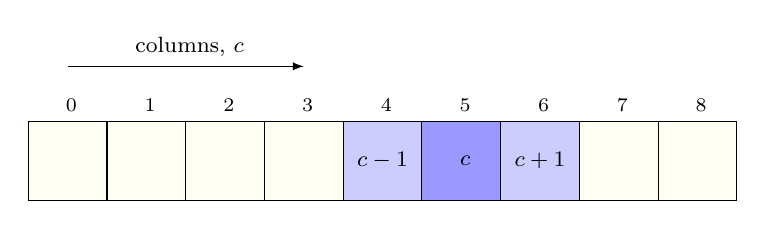
\begin{tikzpicture}

\foreach \c in {0,1,2,...,8} {
	\foreach \r in {0} {
		\node[cell]  at (\c,-\r) {}; 
	}
}
\foreach \c in {0,1,2,...,8} {
	\node at ($(\c,0)+(0,0.7)$) {\smaller[2] \c};
}
\draw[-latex] (0,1.2) -- node[above] {\smaller[1] columns, $c$} ++(3,0);

\node[cell,fill=blue!20] at (6,0) {};\node at (6,0) {\smaller[1]$c+1$};
\node[cell,fill=blue!40] at (5,0) {};\node at (5,0) {\smaller[1] $c$};
\node[cell,fill=blue!20] at (4,0) {};\node at (4,0) {\smaller[1]$c-1$};

\end{tikzpicture}

%: 2D grid 

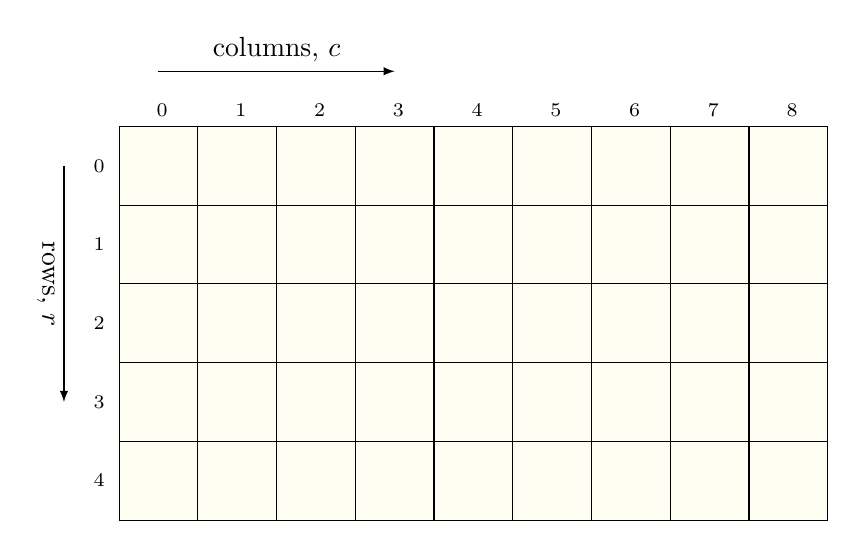
\begin{tikzpicture}

\foreach \c in {0,1,2,...,8} {
	\foreach \r in {0,1,2,...,4} {
		\node[cell]  at (\c,-\r) {}; 
	}
}
\foreach \c in {0,1,2,...,8} {
	\node at ($(\c,0)+(0,0.7)$) {\smaller[2] \c};
}
\foreach \r in {0,1,2,...,4} {
	\node at ($(0,-\r)+(-0.8,0)$) {\smaller[2] \r};
}
\draw[-latex] (0,1.2) -- node[above] {columns, $c$} ++(3,0);
\draw[-latex] (-1.2,0) -- node[below,sloped] {rows, $r$} ++(0,-3);

\end{tikzpicture}

%: 2D grid 

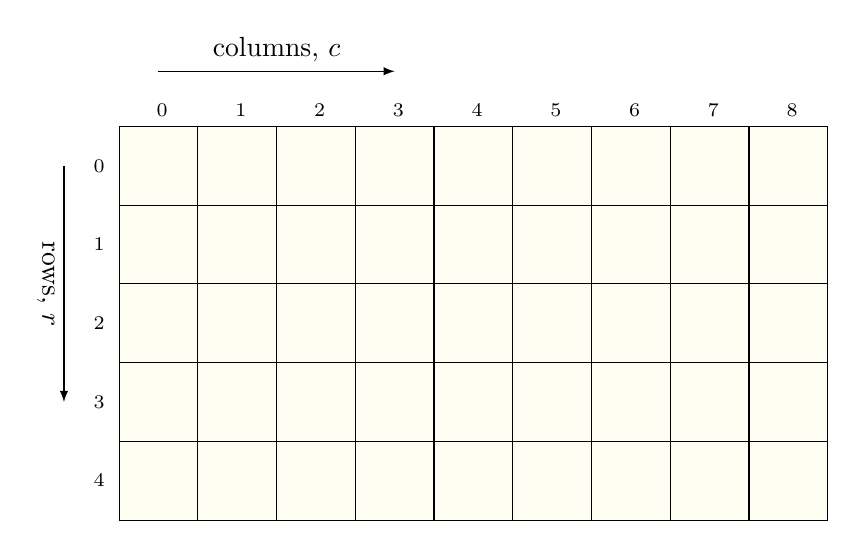
\begin{tikzpicture}

\foreach \c in {0,1,2,...,8} {
	\foreach \r in {0,1,2,...,4} {
		\node[cell]  at (\c,-\r) {}; 
	}
}
\foreach \c in {0,1,2,...,8} {
	\node at ($(\c,0)+(0,0.7)$) {\smaller[2] \c};
}
\foreach \r in {0,1,2,...,4} {
	\node at ($(0,-\r)+(-0.8,0)$) {\smaller[2] \r};
}
\draw[-latex] (0,1.2) -- node[above] {columns, $c$} ++(3,0);
\draw[-latex] (-1.2,0) -- node[below,sloped] {rows, $r$} ++(0,-3);

\end{tikzpicture}

\end{document}
